\chapter{Geometriska vektorer}
    När man säger vektor menar man ofta en matris på formeln av en kolonnvektor, $
    \begin{pmatrix}
        1\\ 2\\ -3
    \end{pmatrix}
    $ eller en radvektor, $\begin{pmatrix}1 & 2 & -3\end{pmatrix}$.
    \\Så kommer det även vara för oss. Men vi börjar med att diskutera geometriska vektorer.

    \paragraph{Definition:} En \underline{geometrisk vektor} är ett objekt som har både storlek och riktning. 
    Storleken av vektorn $\mathbb{V}$ betecknas $||\mathbb{V}||$ och kallas för vektorns längd.
    Det finns en vektor, nollvektorn $\bm{0}$, som har längd 0 men saknar riktining.
    ~\\
    Vi tänker på en geometrisk vektor som en pil $\longrightarrow$
    \\Men en pil har en start- och en slut-punkt. Det har inte vektorer.
    Vektorer vestäms av deras längd och riktning.

    \paragraph{Definition:} Vi säger att \underline{två vektorer är lika} om de har samma längd och samma riktning.
    
    \paragraph{Ex} Vektorerna $\longrightarrow$ och $\rightarrow $ är inte lika för de har inte samma längd.
    De har dock samma riktning.\\
    Vektorerna $\rightarrow  $ och $\downarrow $ är inte lika. De har samma längd (kanske inte blir det i pdf:en) men inte samma riktning.\\
    Vektorerna $\nearrow $ och $\nearrow $ är lika. De har samma längd och samma riktning.
    Start och slutpunkt spelar ingen roll!
    
    \paragraph{Ex} Hastighet är en vektor. I detta fall kallas storleken för fart (speed).
    \par
    ~\\
    Givet två punkter A och B så betecknar $\overrightarrow{AB}$ vektron från A till B. $A\longrightarrow B$
    \\Vi vill kunna räkna med vektorer, dvs göra vektoralgebra.
    
    \clearpage

    \paragraph{Definition:} Givet en vektor $\bm{v}$ och ett tal $a\neq 0$ så är vektorn av den vektorn som uppfyller
    \begin{enumerate}
        \item $||a\cdot \bm{v}||=||a||\cdot ||\bm{v}||$
        \item om $a>0$ då har $a\bm{v}$ och $\bm{v}$ samma riktning
        \item om $a<0$ då har $a\bm{v}$ och $\bm{v}$ motsatt riktning
    \end{enumerate}
    Vi låter $0\cdot \bm{v} = \bm{0} $.
    
    \paragraph{Ex} Om vektorn $\bm{v}$ ges av $\nearrow $ då är $2\bm{v}$, $\frac{1}{2}\bm{v}$ och $(-1)\bm{v}$ vektornerna
    $\nearrow$ (dubbla längden) $\nearrow$ (halva längden) $\swarrow $

    \paragraph{Ex} Om $\bm{v}$ är en vektor med positiv längd, då är $\bm{w}=\frac{1}{||\bm{v}||}$ är en vektor med längd 1.
    Låt oss kolla detta: $||\bm{w}|| = ||\frac{1}{\bm{v}}\bm{v}=|\frac{1}{||\bm{v}||}|\cdot ||\bm{v}||=\frac{1}{||\bm{v}||}||\bm{v}||=1$.\\
    En vektor med längd 1 kallas för en \underline{enhetsvektor}.

    \paragraph{Definition:} Om $\bm{v}=\overrightarrow{AB}$ och $\bm{w}=\overrightarrow{BC}$ då definierar \underline{summan av $\bm{v}$ och $\bm{w}$} som $\bm{v}+\bm{w}=\overrightarrow{AC}$\\
    Illustration:\\
    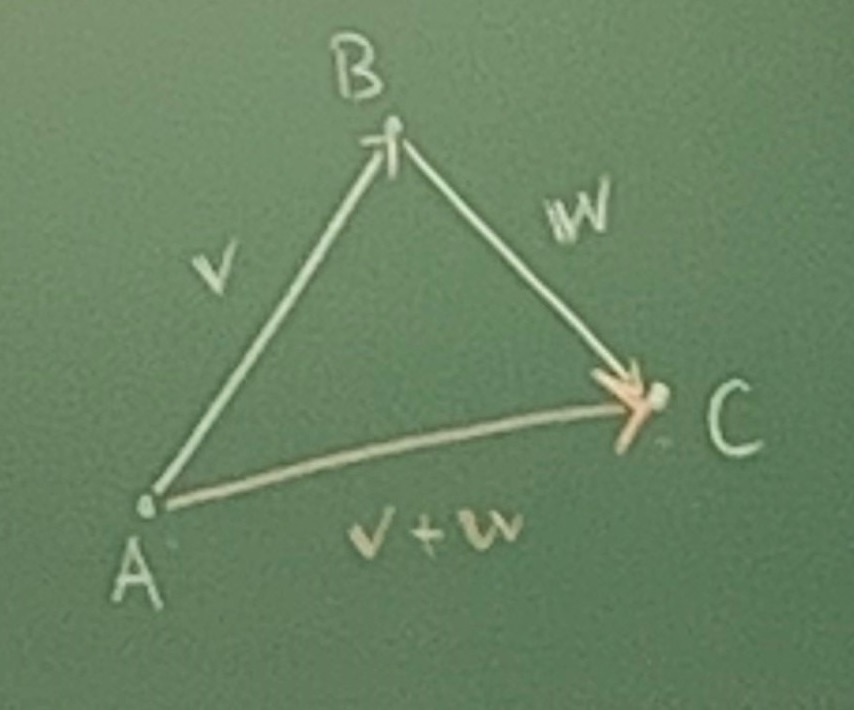
\includegraphics[scale=0.25]{imgs/22-01-17-img01.jpg}
    ~\\      
    Det är ingen inskränkning att anta att $\bm{w}$ börjar där $\bm{v}$ slutar eftersom vi får flytta vektorer.
    
    \subsection{Räkneregler}
    \begin{enumerate}
        \item $a\cdot (b\cdot \bm{v})=(a\cdot b)\cdot \bm{v}$
        \item $(a+b)\bm{v}=a\bm{v}+b\bm{v}$
        \item $a(\bm{v}+\bm{w})=a\bm{v}+a\bm{w}$
        \item $\bm{v}+\bm{w}=\bm{w}\bm{v}$
        \item $\bm{u}+(\bm{v}+\bm{w})=(\bm{u}+\bm{v})+\bm{w}$
    \end{enumerate}
    Räkneregel 5 gör att vi kan skippa paranteser när vi adderar flera vektorer.\\
    Vi skriver $\bm{u}+\bm{v}+\bm{w}$